\chapter{Curbe Eliptice} 

In aceasta capitol vom prezenta conceptul de curba eliptica, pornind de la definitiile de baza, fiind incluse concepte precum structura de grup formata de punctele de pe o curba eliptica, aritmetica din acest grup, aspecte privind ordinul grupului. Vom continua discutia spre aritmetica eficienta, unde vom prezenta algorimi eficienti pentru inmultirea unui punct cu un scalar si pentru inmultire multipla, iar apoi vom discuta despre aplicatii in criptografie (protocolul ECDSA de exemplu). In ultima sectiune voi discuta despre implementarea conceptelor discutate in sectiunile precedente, in acelasi timp facand o comparatie intre algoritmii discutati la sectiunea de aritmetica eficienta.

\section{Introducere}
\label{sec:sec01}

\begin{dfn}
[sursa Guide to elliptic curves menezez]O \textit{curba eliptica} $E$ peste un corp $K$ este definita prin ecuatia:
$$E : y^2 + a_1xy + a_3y = x^3 + a_2x^{2} + a_4x + a_6$$ 
\\unde $a_1, a_2, a_3, a_4, a_5, a_6\in K$, iar discriminantul ecuatiei, $\Delta \neq 0$. Discriminantul ecuatiei este definit astfel:
$$ \begin{cases}
\Delta = -d_2^{2}d_8 - 8d_4^{3} - 27d_6^{2} + 9d_2d_4d_6 \\
d_2 = a_1^{2} + 4a_2 \\
d_4 = 2a_4 + a_1a_3 \\
d_6 = a_3^{2} + 4a_6 \\
d_8 = a_1^{2}a_6 + 4a_2a_6 - a_1a_3a_4 + a_2a_3^{2} - a_4^{2}
\end{cases}$$
\end{dfn}
\begin{dfn}
Fie $L$ orice extensie a corpului $K$. Definim multimea de $L$-puncte rationale peste $E$ astfel: $E(L) = \set {(x, y)\in L\times L: y^2 + a_1xy + a_3y - x^3 - a_2x^{2} - a_4x - a_6 = 0} \cup \set {\infty}$
\end{dfn}
\begin{obs}
In urmatoarele randuri voi face o serie de observatii asupra ecuatiei unei curbe eliptice: \\
(i) Ecuatia de la definitia 2.1 se numeste Ecuatie Weierstrass \\
(ii) Conditia ca discriminantul $\Delta$ sa fie diferit de 0 asigura "netezimea" curbei eliptice, adica nu exista puncte care sa aibe 2 sau mai multe tangente diferite la curba. \\
(iii) L-punctele rationale sunt acele puncte, $(x, y)$ care satisfac ecuatia Weierstrass, cu $x, y \in L$. Punctul de la infinit este considerat un punct L-rational pentru toate extensiile $L$ ale corpului $K$
\end{obs}

\begin{dfn}
Fie $E_1, E_2$ doua curbe eliptice, definite astfel: \\
$E_1 : y^2 + a_1xy + a_3y = x^3 + a_2x^{2} + a_4x + a_6$ \\
$E_2 : y^2 + \overline{a_1}xy + \overline{a_3}y = x^3 + \overline{a_2}x^{2} + \overline{a_4}x + \overline{a_6} $ \\
Spunem ca cele doua curbe sunt \textit{izomorfe} daca exista $u,r,s,t\in K, u\neq 0$ astfel incat schimbarea de variabila $(x, y)\rightarrow (u^2x + r, u^3y + u^2sx + t)$ transforma ecuatia $E_1$ in ecuatia $E_2$. Acest tip de transformare se numeste schimbare "admisibila" de variabila.
\end{dfn}
\begin{dfn}
Ecuatia Weierstrass a unei curbe eliptice poate fi simplificata in mod considerabil, aplicand schimbari admisibile de variabila. Vom trata trei cazuri separate de schimbari de variabila, in functie de caracteristica corpului $K$, ajungand la o forma \textit{simplificata a Ecuatiei Weierstrass.}. Vom aborda trei cazuri, primul fiind $char(K) \neq \set {2,3}$ \\

  1. Fie $K$ un corp si \textit{E} o curba eliptica data prin ecuatia lui Weierstrass. O schimbare admisibila de variabila este:
$(x, y) \rightarrow (\frac{x - 3a_1^{2} - 12a_2}{36}, \frac{y-3a_1x}{216} - \frac{a_1^{3} + 4a_1a_2 - 12a_3}{24})$ \\
Aceasta schimbare transforma ecuatia $E$ in ecuatia 
\begin{center} $y^2 = x^3 + ax + b; a, b\in K$\end{center}
Discriminantul acestei noi ecuatii este $\Delta = -16(4a^3 + 27b^2)$ \\

2. Daca $char(K) = 2$ trebuie sa consideram doua subcazuri. Daca $a_1 \neq 0$, atunci o schimbare admisibila de variabila este: $(x, y) \rightarrow (a_1^2x + \frac{a_3}{a_1}, a_1^3y + \frac{a_1^2a_4 + a_3^2}{a_1^3} )$, care transforma $E$ in:
\begin{center}$y^2 + xy = x^3 + ax^2 + b; a, b\in K$\end{center}
O astfel de ecuatie se numeste \textit{non-supersingulara} si are discriminantul $\Delta = b$ \\
Daca $a_1 = 0$ atunci o schimbare admisibila ar fi $(x, y)\rightarrow (x + a_2, y)$ care transforma curba $E$ in
\begin{center} $y^2 + cy = x^3 + ax + b; a,b,c\in K$ \end{center}
O astfel de ecuatie se numeste \textit{supersingulara} si are discriminantul $\Delta = c^4$
\\

3. Daca $char(K) = 3$ trebuie sa consideram din nou doua subcazuri. Daca $a_1^2 \neq -a_2$ atunci o schimbare admisibila de variabila este
$(x, y) \rightarrow (x + \frac{\alpha}{\beta}, y + a_1x + a_1\frac{\alpha}{\beta} + a_3)$, unde $\alpha = a_4 -a_1a_3$ si $\beta = a_1^2 - a_2$. Ecuatia $E$ devine: 
\begin{center} $y^2 = x^3 + ax^2 + b; a, b\in K$\end{center}
O astfel de ecuatie se numeste \textit{non-supersingulara} si are discriminantul $\Delta = -a^3b$ \\
Daca $a_1^2 = -a_2$ atunci consideram o schimbare admisibila de variabila $(x, y) \rightarrow (x, y + a_1x + a_3)$ care transforma curba $E$ in:
\begin{center} $y^2 = x^3 + ax + b$ \end{center}
O astfel de curba este \textit{supersingulara} si are discriminantul $\Delta = -a^3$
\end{dfn}

\begin{obs}
Vom lucra cu forma simplificata a ecuatiei Weierstrass pe tot parcursul urmatoarelor capitole.
\end{obs}

\subsection{Grupul punctelor de pe o curba eliptica}
\label{subsec:subsec01}
Fie $E$ o curba eliptica in forma Weierstrass peste un corp $F_q$. Punctele care apartin acestei curbe formeaza o structura de grup abelian, acestea respectand regulile unei astfel de structuri

\begin{itemize}
  \item Definim elementul netru in grup ca fiind punctul de la infinit, notat $\infty$. Astfel, pentru orice punct $P$ de pe curba, avem: $P + \infty = \infty + P$
  \item Fie $P(x, y)\in E(F_q)$. Atunci exista $-P = (x, -y) \in E(F_q)$ astfel incat $P+ (-P) = \infty$. Numim $-P$, inversul punctului $P$. De asemenea, avem $\infty = -\infty$
  \item Oricare ar fi doua puncte, $P, Q\in E(F_q)$, avem $P + Q \in E(F_q)$. In continuare vom defini aceasta operatie de adunare mai in detaliu.
\end{itemize}

\begin{dfn}
Adunarea a doua puncte de pe o curba eliptica este foarte intuitiva din punct de vedere geometric. Fie $P, Q$ doua puncte si $R$ suma lor. Rezultatul este obtinut astfel. Mai intai desenam o linie intre $P, Q$. Acesta linie intersecteaza curba intr-ul al treilea punct. Punctul $R$ este reflectia la axa $Ox$ a acestui punct(Figura 2.1a). Dublul unui punct $P(2P = R)$ este definit astfel. Desenam o tangenta la curba eliptica in P, aceasta intersectand curba intr-un punct secundar. Punctul $R$ este din nou reflexia la axa $Ox$(Figura 2.1b).  
\end{dfn}

\begin{obs}
Formulele algebrice pentru adunarea a doua puncte difera in functie de sistemul de coordnate folosit, sau tipul de corp algebric peste care este definita curba eliptica(corp prim, binar sau de extensie).
\end{obs}

\begin{figure}[htp]
\centering
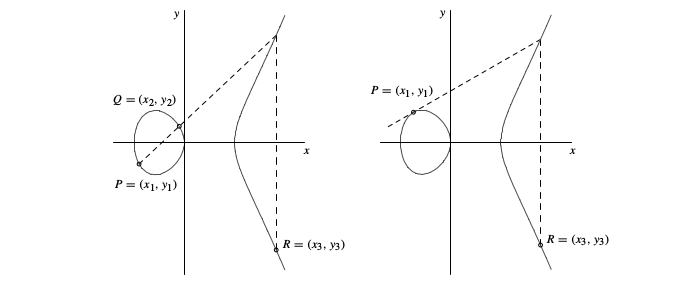
\includegraphics[width=13cm]{chapters/Addition.png}
\caption{Adunarea si dublarea unui punct pe o curba eliptica}
\label{fig:lion}
\end{figure}

\begin{dfn}
Pentru puncte reprezentate prin coordonate afine formulele de calcul sunt dupa cum urmeaza.Fie doua puncte, $P(x_{1}, y_1), Q(x_2, y_2)\in E(F_p)$. Notam cu $R(x_3, y_3) = P + Q$. Formulele pentru adunarea a doua puncte pot fi demonstrate matematic destul de usor, pornind de la ideea ca $P, Q$ si simetricul rezultatului fata de axa $Ox$ se afla pe aceasi dreapta, respectiv pe aceasi curba eliptica.

$\begin{cases} 
    x_3 = \lambda^2 - x_1 - x_2 \\
    y_3 =  \lambda (x_1-x_3) - y_1
   \end{cases}$
 \\cu 
 \\$
 \lambda = 
 \begin{cases}
 \frac{y_2 - y_1}{x_2 - x_1}, P \neq Q \\ 
 \frac{3x^{2}_1 + a}{2y_1}, P = Q
 \end{cases}$ \\
\end{dfn}

\begin{dem}
Fie $P(x_1, y_1), Q(x_2, y_2)\in E(F_p)$ Punctele se afla pe aceasi dreapta. Scriind ecuatia dreptei care trece prin cele doua puncte si considerand ca $-R\in E(F_p)$, rezolvam sistemul de ecuatii:
$\begin{cases} 
    0 = \begin{vmatrix}
			x_1 & y_1 & 1 \\ 
			x_2 & y_2 & 1 \\ 
			x & y & 1  \\ 
			\end{vmatrix} \\
    y^2 =  x^3 + ax + b
   \end{cases}$
   Panta dreptei este $\lambda = \begin{cases}
 \frac{y_2 - y_1}{x_2 - x_1}, P \neq Q \\ 
 \frac{3x^{2}_1 + a}{2y_1}, P = Q
 \end{cases}$
 \\Inlocuind in formula curbei eliptice obtinem formulele din definita precedenta.
\end{dem}

\subsection{Constructia curbelor eliptice}
\label{subsec:subsec02}

Fie $E$ o curba eliptica peste un corp $K = F_q$. Asa cum am vazut in sectiunea anterioara, multimea de puncte $E(F_q)$ impreuna cu operatia de adunare formeaza o structura de grup abelian, cu punctul de la infinit fiind elementul neutru din grup. Acest grup este folosit in criptografia bazata pe curbe eliptice.


\begin{dfn}
Numim \textit{ordin} al unei curbe eliptice, numarul de puncte care satisfac ecuatia Weierstrass, cu alte cuvinte cardinalul multimii $E(F_q)$ si il notam cu $\# E(F_q)$. Teorema care urmeaza, datorata lui \textit{Hasse}, ofera o aproximare pentru acest ordin
\end{dfn}
\begin{teo}
Fie $E$ o curba eliptica definita peste $F_q$. Atunci este adevarata relatia:
\begin{center} $q + 1 - 2\sqrt{q}\leq \# E(F_q)\leq q+1 + 2\sqrt{q}$ \end{center}
Intrucat $2\sqrt{q}$ este relativ mic in comparatie cu $q$, putem afirma ca $\# E(F_q) \approx q$
\end{teo}
\begin{teo}
Fie $q = p^m$, unde $p$ este caracteristica corpului $F_q$. Atunci exista o curba eliptica $E$ definita peste acest corp, cu $\# E(F_q) = q+1-t$ ($t$ se numeste urma curbei eliptice $E$) daca si numai daca una dintre urmatoarele conditii este adevarata: \\
(i) $t \not\equiv 0$ mod $p$ si $t^2\leq 4q$ \\
(ii) m este impar si $t=0$ sau $t^2 = 2q$ si $p=2$ sau $t^2 = 3q$ si $p=3$ \\ 
(iii) m este par si $t^2 = 4q$ sau $t^2 = q$ si $p\not\equiv 1$ mod $3$ sau $t= 0$ si $p\not\equiv 1$ mod $4$
\end{teo}
\begin{dfn}
Fie $p$ caracteristica corpului $F_q$. Numim curba eliptica \textit{supersingulara}, daca $p$ divide $t$, unde t este urma curbei. Altfel, curba $E$ este \textit{non-supersingulara}
\end{dfn}
\begin{teo}
Fie $E$ o curba eliptica peste corpul $F_q$ si fie ordinul acesteia $\# E(F_q)= q+ 1-t$. Atunci, $\# E(F_q) = q+ 1 - V_n$, unde definim sirul $\set {V_n}$ recursiv prin formula $V_0 = 2, V_1=t$ si $V_n = V_1V_{n-1} - qV_{n-2}, \forall n\geq 2$
\end{teo}
Urmatoarea teorema descrie structura grupului pentru o curba eliptica. Vom nota un grup ciclic de ordin n, cu $Z_n$.
\begin{teo}
Fie E o curba eliptica definita peste $F_q$. Atunci grupul $E(F_q)$ este izomorfic cu $Z_{n_1} \oplus Z_{n_2}$, unde $n_1, n_2\in Z$, unici determinati, cu $n_2$ care divide atat $n_1$ cat si $q-1$. Daca $n_2=1$, spunem ca $E(F_q)$ este grup ciclic.
\end{teo}

\subsection{Reprezentari ale punctelor de pe o curba eliptica}
\label{subsec:subsec03}
De multe ori, in efectuarea operatiile pe curbe eliptice, poate fi avantajos sa reprezentam un punct in alte coordonate decat cele afine(sectiunea 2.3.1). De exemplu, in calculul sumei a doua puncte(operatie care la randul ei este folosita in algoritmii pentru inmultirea cu un scalar si in inmultirea multipla) se observa necesitatea de a efectua operatia de invers modular de mai multe ori. Acesta operatie este costisitoare din punct de vedere computational, astfel vom folosi diferite tipuri de reprezentari.
\begin{dfn}
Fie $K$ un corp si $c, d\in \mathbb{N}$. Definim o relatie de echivalenta peste multimea $K^3\setminus \set {(0, 0, 0)}$ ca fiind :
\begin{center} $(X_1, Y_1, Z_1) \equiv (X_2, Y_2, Z_2)$ daca $X_1 = \lambda ^cX_2, Y_1 = \lambda ^d Y_2, Z_1 = \lambda Z_2, \lambda\in K^{*}$\end{center}
Exista o corespondenta $1-1$ intre multimea de puncte in coordonate proiective $P(K)^{*} = \set {(X, Y, Z): X, Y, Z\in K, Z\neq 0}$ si multimea punctelor in coordonate afine, $A(K) = \set {(x, y): x, y\in K}$
\end{dfn}
\begin{dfn}
Consideram $c=1, d=1$ in definitia \textit{coordonatelor proiective}. Acestea se numesc \textit{coordonate proiective standard}. Punctu l in coordonate proiective $(X, Y, Z), Z\neq 0$ corespunde punctului in coordonate afine $(X/Z, Y/Z)$. Ecuatia curbei eliptice devine:
\begin{center}  $Y^2Z = X^3 + aXZ^2 + bZ^3$ \end{center}
Punctul de la infinit este $(0, 1, 0)$ in timp ce inversul unui punct oarecare este $(X, -Y, Z)$
\end{dfn}
\begin{dfn}
Consideram $c=2, d=3$. Acest sistem de coordonate se numesc coordonate \textit{proiective Jacobi}. Punctul $(X, Y, Z), Z\neq 0$ corespunde punctului 
in coordonate afine $(X/Z^2, Y/Z^3)$. Ecuatia curbei devine:
\begin{center} $Y^2 = X^3 + aXZ^4 + bZ^6$ \end{center}
Punctul de la infinit este $(1, 1, 0)$, iar inversul unui punct este $(X, -Y, Z)$
\end{dfn}
\begin{dfn}
\textit{Coordonatele Chudnovsky} sunt obtinute din coordonatele Jacobi, adaugand niste reduntante. Astfel, un punct reprezentat in acest tip de coordonate, arata in acest fel : $(X, Y, Z, Z^2, Z^3)$. Acest tip de reprezentare aduce imbunatatiri de performanta cand folosim anumiti algoritmi specializati pentru inmultirea cu un scalar.
\end{dfn}

\begin{obs}
Se poate folosi $Z = 1$ in implementari pentru a simplifica calculele.
\end{obs}

\section{Aritmetica eficienta}
\label{sec:sec02}

In aceasta sectiune vom face o prezentare a metodelor eficiente de inmultire cu un scalar si de inmultire multipla. Printre metodele de inmultire cu un scalar, se numara algoritmul binar, algoritmul care foloseste o reprezentare cu semn a scalarului si diferite metode de inmultire cu fereastra. La inmultirea multipla, avem un algoritm naiv si doua metode de inmultire eficienta. 

\subsection{Inmultirea cu un scalar}

\begin{dfn}
Definim operatia de inmultire a unui punct $P$ de pe o curba eliptica, cu un scalar, $k\in \mathbb{Z}$, notata cu $kP$, ca fiind: \\
- $0P = \infty$ \\
- $(k+1)P = kP + P, k\geq 0$ \\
- $kP = -|k|P, k < 0$ \\
Exista multe metode de a face acest lucru, de la metoda brute force de a face k adunari repetate ($kP = P+P+\cdots +P$) pana la metode mai rafinate, precum cea a ferestrei glisante, care inbunatatesc considerabil performanta operatiei. Vom discuta in continuare despre diferite metode eficiente pentru aceasta operatie.
\end{dfn}

\subsubsection{Metoda Binara}

Metoda naiva de a inmulti un punct cu un scalar, cea prezentata in definitie, necesita $k-1$ adunari pentru a calcula $kP$. O prima optimizare este data de aceasta metoda binara, care necesita cel mult $m$ adunari (sursa Silverman, second edition) si in medie $m/2$ adunari, unde $m$ este numarul de biti din reprezentarea lui $k$. Algoritmul consta in procesarea de la dreapta la stanga, sau de la stanga la dreapta a scalarului. Dupa fiecare bit parcurs dublam resultatul si cand intalnim un bit de $1$ adunam punctul $P$ la resultat. Astfel, dupa parcurgerea a $\log_2 k$ iteratii(numarul de biti din reprezentarea lui $k$) avem rezultatul.

\begin{ex}
Fie curba eliptica $E: y^2 = x^3 + 3x + 2$, punctul $P(10, 16)\in E$ si un scalar $d = 5$. Reprezentarea binara a scalarului este $d = (1, 0, 1)$. Asadar resultatul va fi egal cu: $r = (10, 16) + 4*(10, 16)$. Am adunat la rezultat $P$ deoarece cel mai nesimnificativ bit este 1, apoi am dublat $P$ de 2 ori(2 biti parcursi) si l-am adunat la rezultat deoarece bitul cel mai semnificativ este $1$. Astfel obtinem $5P = (66, 73)$
\end{ex}

\subsubsection{Reprezentari cu semn}

Un avantaj major al curbelor eliptice, este faptul ca in grupul format de punctele de pe o astfel de curba, operatia de invers este foarte eficienta. Astfel, daca consideram 2 puncte $P, Q$ intr-un astfel de grup, putem calcula $P + Q$ si $P - Q$ cu aproximativ acelasi cost computational. Aceasta observatie este foarte importanta in eficientizarea algoritmilor de inmultire cu un scalar. Calculul inversului avand un cost neglijabil din punct de vedere computational, nu este necesar sa ne limitam la $\set{0, 1}$ in reprezentarea unui scalar. Introducem astfel conceptul de reprezentare cu semn.

\begin{dfn}
[Sursa: Solinas] Fie $n\in\mathbb{N}$. O reprezentare a lui cu semn poate fi notata astfel: $n = <u_{l-1}u_{l-2}...u_1u_0>$, unde $u_i\in\set{0, -1, 1}$. Astfel $n = \sum_{i=0}^{l-1} u_i 2^{i}$. Exista o infinitate de astfel de reprezentari.
\end{dfn}
\begin{dfn}
Reprezentarea cu semn optima pentru operatia de inmultire cu un scalar este asa numita NAF, sau Non Adjacent Form. Aceasta are proprietatea ca nu exista doua elemente consecutive din reprezentarea cu semn diferite de 0.
\end{dfn}

\begin{teo}
NAF-ul are urmatoarele proprietati:
\begin{itemize}
  \item Orice numar natural are un NAF
  \item NAF-ul unui numar este unic
  \item Lungimea NAF-ului unui numar natural este cu cel mult o unitate mai mare decat expansiunea binara a numarului 
  \item NAF-ul are distanta Hamming minima dintre toate reprezentarile cu semn
\end{itemize}
\end{teo}

Un algoritm care foloseste aceasta reprezentare a scalarului, functioneaza asemanator cu cel de la metoda binara. Parcurgem reprezentarea cu semn, dublam resultatul dupa fiecare bit parcurs, adunam $P$ cand intalnim un bit de $1$ si scadem $P$ cand intalnim un bit de $-1$. Aceasta metoda necesita in medie $m/3$ adunari si $m$ dublari, unde m reprezinta numarul de biti din reprezentarea scalarului (sursa Menezez).

\begin{ex}
Fie curba eliptica $E: y^2 = x^3 + 3x + 2$, punctul $P(10, 16)\in E$ si un scalar $d = 5$. Reprezentarea cu semn a lui d este, $d = (1, 0, 0, -1)$. Parcurgem de dreapta la stanga resultatul, si avem dupa prima iteratie $resultat = P$. Dupa a doua iteratie $resultat = 2P$. Dupa a treia iteratie $resultat = 4P$, iar la ultima iteratie, $resultat= 8P - P= 7P$. Asadar $7P = (14, 13)$
\end{ex}

\subsubsection{Metoda cu fereastra}

Algoritmii care se folososesc de reprezentarea cu semn a scalarului pot fi inbunatatiti daca avem disponibila mai multa memorie. Vom procesa $w$ cifre din scalar la o iteratie, unde $w$ reprezinta latimea ferestrei.

\begin{dfn}
Fie $w\geq 2$ un numar natural. Numim o reprezentare NAF de latime $w$ pentru un scalar $n\in\mathbb{N}$, notata cu $w-NAF$, un sir de numere $n = <u_{l-1}u_{l-2}...u_1u_0>$ astfel incat $|u_i| < 2^{w-1}$ si $n = \sum_{0}^{l-1}u_i2^i$ astfel incat cel mult una din $w$ cifre consecutive din sir este diferita de 0.
\end{dfn}

\begin{teo}
Urmatoarele proprietati sunt adevarate pentru $w-NAF$:
\begin{itemize}
\item $2-NAF = NAF$ pentru orice numar $k\in\mathbb{N}$
\item $w-NAF$ unui numar este unic
\item Reprezentarea $w-NAF$ este cu cel mult un bit mai mare decar reprezentarea binara a unui numar
\item Densitatea medie a cifrelor diferite de $0$ din reprezentarea $w-NAF$ de lungime $l$ a unui numar este $\frac{1}{w+1}$
\end{itemize}
\end{teo}

Algoritmul care calculeaza $nP$ folosind aceasta metoda este asemanator cu algoritmii precedenti, dar folosim aceasta reprezentare $w-NAF$ pentru scalar. Fie $n = <u_{l-1}u_{l-2}...u_1u_0>$ reprezentarea $w-NAF$ a unui numar natural $n$. Dorim sa calculam $nP$. Algoritmul nostru parcurge fiecare numar din reprezentarea $w-NAF$ dubland rezultatul dupa fiecare iteratie, adunand sau scazand $u_iP$ la resultat, $i\in \set{0, l-1}$. Valoarea lui $u_iP$ este precalculata si stocata. \\

Conform teoremei $2.6$, numarul mediu de adunari si dublari pentru algoritmul prezentat mai sus este $[1D + (2^{w-2} - 1) A] + [\frac{m}{w+1}A + mD]$, unde $m = \log_2 n$, $A$ reprezinta adunare si $D$ dublare. [sursa Menezes]

\begin{ex}
Fie curba eliptica $E: y^2 = x^3 + 3x + 2$, punctul $P(10, 16)\in E$, un scalar $d = 39$ si lungimea ferestrei $w=3$. Reprezentarea $3-NAF$ pentru d este $(1, 0, 0, -3, 0, 0, -1)$. Vom precalcula si stoca valorile pentru $(P, 3P)$, iar apoi parcurgem $3-NAF$ de la stanga la dreapta. Initiem variabila rezultat cu "punctul de la infinit", iar dupa fiecare iteratie, in rezultat vom avea: $P, 2P, 4P, 5P, 10P, 20P, 39P$. Dupa fiecare bit parcurs, am dublat rezultatul, am scazut $-3P$ la iteratia 4 si $-P$ la ultima iteratie. Ambele valori erau precalculate. La final, avem $resultat = 39P = (60, 39)$

\end{ex}

\subsubsection{Metoda cu fereastra glisanta}

    Pentru a eficientiza metoda cu fereastra fixa prezentata mai sus, vom procesa folosi o asa zisa "fereastra glisanta" asupra cifrelor din $w-NAF$. Ideea e sa folosim o fereastra de lungime $w$ pe care o "glisam" (procesam mai mult decat o singura cifra din $w-NAF$) peste reprezentarea scalarului. Mentinem intotdeauna o valoarea impara in fereastra pentru a micsora numarul de precalculari necasar. La fiecare iteratie, cand gasim o cifra diferita de $0$ in $w-NAF$, cautam cel mai mare $t \leq w$ valoarea numarului dat de $w-NAF$ de lungime t este impara. Adunam sau scadem la resulatat acea valoare apoi "glisam" fereastra la dreapta cu $t$ pozitii.
\begin{obs}
Numarul mediu de zerouri intre ferestre este egal cu:
$$\nu(w) = \frac{4}{3} - \frac{(-1)^w}{3\times 2^{w-2}}$$
Astfel, numarul mediu de adunari si dublari al algoritmul cu fereastra glisanta este:
$$[1D + (\frac{2^w - (-1)^w}{3} - 1)A] + \frac{m}{w + \nu(w)}A + mD$$
[sursa Menezes]
\end{obs}

\begin{ex}
Vom folosi acelasi exemplu ca la Metoda cu fereastra clasica, aceasi curba, acelasi fereastra, acelasi punct si acelasi scalar. Algoritmul il aplicam de la stanga la dreapta pe $3-NAF$ al punctului $P$. La fiecare iteratie avem nevoie de o variabila $t$ care da diminesiunea ferestrei, si $u$, valoarea in fereastra. Dupa fiecare iteratie, vom avea: $s=1, u=1, resultat=P; resultat = 2P; resultat = 4P; s=4, u=-3, resultat = 5P; resultat = 10P; resultat = 20P; s=6, u=-1, resultat=39P$. La final, avem in $39P = (60, 39)$
\end{ex}

\subsection{Inmultirea multipla}

\begin{dfn}
O operatie asemanatoare celei de inmultire cu un scalar, este cea de inmultire multipla cu scalari. Fie doua puncte, $P, Q$ de pe o curba eliptica si doi scalari, $k, l\in \mathbb{Z}$. Dorim sa aflam rezultatul $kP + lQ$. Evident, precum la operatia de inmultire cu un scalar putem aplica o metoda directa, de a inmulti punctul $P$ cu scalarul $k$ respectiv punctul $Q$ cu scalarul $l$ si apoi facem o adunare de puncte. Acest lucru este insa ineficient, intrucat exista si aici metode mai rapide de a calcula acest lucru. Aceasta operatie de inmultire rapida este una extrem de folosita in criptografia pe curbe eliptice, aparand de exemplu, in cadrul unor protocoale criptografice, precum ECDSA, iar implementarea ineficienta e acesteia duce la mari probleme de performanta. 
\end{dfn}

\subsubsection{Metoda naiva}
O prima metoda de a aborda calculul $kP + lQ$ se bazeaza pe metode deja discutate. Calculam separat $kP$ si $lQ$, folosind unii din algorimii precizati la sectiunea anterioara, apoi adunam rezultatele. Aceasta metoda este ineficienta, facand multe adunari si dublari redundante.

\begin{ex}
Fie doua puncte, $P(10, 16), Q(14, 13)\in E$, unde $E: y^2 = x^3 + 3x + 2$. Cautam rezultatul $5P + 6Q$. Folosim metoda binara pentru a gasi resultatele $5P = (66, 73)$ si
$6Q = (89, 57)$ apoi vom face adunarea $(66, 73) + (89, 57) = (36, 20)$
\end{ex}

\subsubsection{Representarea Joint Sparse Form}

\begin{dfn}

Consideram 2 reprezentari cu semn pentru scalarii care apar in calculul $kP + lQ$. Combinam aceste 2 reprezentari intr-o singura reprezentare, pe care o vom numi reprezentare reunita. Astfel, daca consideram 2 reprezentari cu semn pentru $k, p$ ca fiind $<u_{l-1}u_{l-2}...u_1u_0>$ respectiv $<v_{l-1}v_{l-2}...v_1v_0>$, reprezentarea lor reunita este $(<u_{l-1}u_{l-2}...u_1u_0>, <v_{l-1}v_{l-2}...v_1v_0>)$. Exista multe astfel de reprezentari, dar cea mai eficienta este asa numita Joint Sparse Form ([Solinas]) care are urmatoarele proprietati:
\begin{itemize}
\item Pentru oricare 3 pozitii consecutive, cel putin una este $0, 0$. Altfel spus, oricare ar fi $i, j\in\mathbb{N}$ avem $u_{i, j+k} = u_{1-i, j+k} = 0, k=0,\pm 1$
\item Termeni adiacenti nu pot avea semne diferite. Astfel, nu putem avea egalitatea $u_{i, j+1}u_{i, j} = -1$
\item Daca $u_{i, j+1}u_{i, j}\neq 0 \Rightarrow u_{1-i, j+1} = \pm 1$ si $u_{1-i, j}=0$
\end{itemize}
\end{dfn}

\begin{ex}
Fie scalarii $21, 26$. Reprezentarea lor Joint Sparse Form este data de:
$$<1, 0, -1, 0, -1, -1>$$
$$<1, 0, -1, 0, 1, 0>$$
\end{ex}

Algoritmul care foloseste aceasta reprezentare se numeste "Shamir's Trick" si calculeaza $kP + lQ$ astfel. Precalculeaza $P, Q, -P, -Q, P + Q, P - Q, -P - Q$ si in functie de cifrele care apar in parcurgerea reprezentarii Joint Sparse adauga la resultat una din valori. De exemplu daca la o iteratie avem combinatia $1, 1$ adaugam $P + Q$, daca avem $-1, -1$ adaugam $-P - Q$, etc. In continuare vom prezenta un exemplu de calcul cu acest algoritm.

\begin{ex}
Fie curba eliptica si punctele de la exemplul precedent, dar de aceasta data vom alege scalarii $d = 21, l = 26$. Vrem asadar sa calculam rezultatul $dP + lQ$ folosind metoda Joint Sparse Form. Mai intai trebuie sa calculam JSF pentru cei doi scalar, rezultatul fiind $(1, 0, -1, 0, -1, -1), (1, 0, -1, 0, 1, 0)$. Vom crea o variabila $resultat$ in care la fiecare iteratie vom avea in variabila resultat urmatoarele: $resultat = P + Q; resultat = 2P + 2Q; resultat = 3P + 3Q; resultat = 6P + 6Q; resultat = 11P + 13Q; resultat = 21P + 26P = (48, 35)$.

\end{ex}

\subsubsection{Metoda cu fereastră glisantă intercalată}

Spre deosibire de metada precedentă de calcul, ideea aici este să facem pentru fiecare punct în parte precalculul separat, dar pasul de dublare trebuie făcut simulatan. Putem folosi ferestre de dimensiuni diferite pentru fiecare scalar în parte, calculând $w-NAF$ lor. În faza de precalcul, stocăm pentru fiecare punct $iP, i<2^{w-1}$, $i$ impar. Reprezentările $w-NAF$ ale punctelor sunt procesate simultan de la stânga la dreapta, cu o singură variabilă $Q$ pe post de rezultat, care se dublează la fiecare iterație. Putem vizualiza ce se întâmplă cu această variabilă la fiecare iterație  în figura 2.2.

\begin{figure}[htp]
\centering
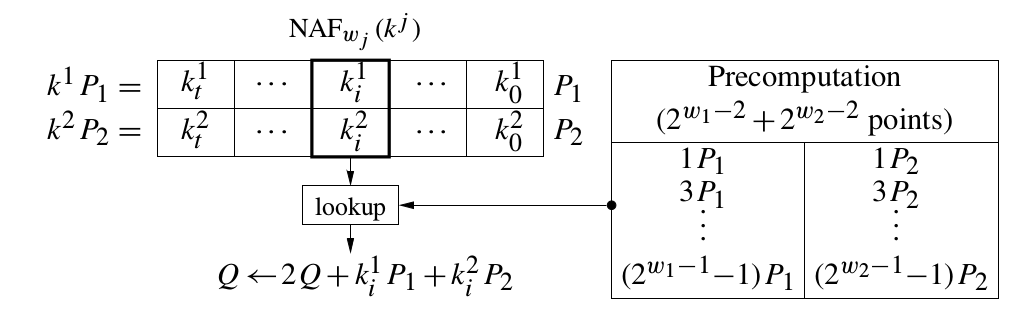
\includegraphics[width=10cm]{chapters/interleaving.png}
\caption{Variabila rezultat la o iterație oarecare}
\label{fig:lion}
\end{figure}

\begin{obs}

Conform \cite{interleaving} Numărul mediu de adunari si dublări este:
$$[|\set{j:w_j>2}|D+\sum_{j=1}^{2}(2^{w_j-2}-1)A]+[\max_{1\leq j\leq 2} l_jD + \sum_{j=1}^{2}\frac{l_j}{w_j+1}A]$$
\end{obs}

\begin{ex}
Păstrând curba si punctele de la exemplele precedente, dorim sa calculam $10P + 41Q$, cu ferestrele $4, 4$. Trebuie asadar sa calculam $4-NAF$ pentru cei doi scalari. Obtinem $(5, 0), (3, 0, 0, 0, -7)$. Padam cu 0 astfel incat cele doua reprezentari sa aiba lungimi egale, obinand astfel $(0, 0, 0, 5, 0), (3, 0, 0, 0, -7)$. Dupa fiecare iteratie, in variabila $resultat$ avem: $resultat = 3Q; resultat = 6Q, resultat=12Q, resultat = 5P + 24Q; resultat = 10P + 41Q = (8, 21)$.
\end{ex}


\begin{obs}
Operatia de adunare pe o curba eliptica este corespondenta operatiei de inmultire
in sistemele cu chei publice obisnuite, iar adunarea multipla este corespondenta
exponentierii modulare din acestea.
Desi regulile de calcul in grupul punctelor unei curbe eliptice par destul de complicate, aritmetica acestora poate fi implementata extrem de eflcient, calculele in acest grup fiind realizate mult mai rapid decat cele din grupul $Z_p$, deoarece operatia de invers este una necostisitoare din punct de vedere computational.
\end{obs}




